
\chapter{Viability Analysis}


\section{Introduction to Performance Testing}

\subsection{Purpose of Testing}


Performance testing is crucial in assessing the viability of the Python implementation of the Ataccama Expression Language, particularly in ensuring it can efficiently and effectively handle data quality rules within Python environments. This testing is not about matching the performance of similar solutions - Soda Core and Great Expectations -  but rather ensuring that the Python version is sufficiently efficient for practical use. The aim is to determine if the Python implementation performs within acceptable limits, where a slowdown by a factor of up to 10 times compared to the similar solutions might be considered tolerable for deployment, but a 1000 times slowdown would indicate serious efficiency issues that could render the solution impractical. By establishing these performance benchmarks, we can validate that the Python implementation meets minimum requirements for real-world applications, ensuring it is a viable alternative for data engineers who require programmatic access to Ataccama's data quality tools.

\subsection{Testing Framework}

\subsubsection{Tools and Setup}

The performance testing utilizes a structured approach where a specific data quality rule—represented in three different formats: an original Ataccama expression, a Soda Core implementation, and a Great Expectations setup—is executed across a range of dataset sizes. This method allows for a direct comparison of how well the Python implementation scales with increasing data volumes, a critical factor in many data engineering tasks.

\subsubsection{Methodology}

\paragraph{Dataset Sizes} Tests are conducted on datasets of varying sizes, starting from 10 records and scaling up to 1 or 10 million records depending on test case complexity. This range is chosen to simulate different real-world scenarios, from small, manageable datasets to large-scale data processing tasks.

\paragraph{Execution Repetition} Each test is repeated ten times to ensure consistency and reliability in the results. This repetition helps mitigate any anomalies or outliers that could affect the accuracy of the performance assessment.
The first repetition is considered a warm-up to allow the Python interpreter to optimize the code before the actual performance metrics are recorded. This approach ensures that the performance measurements are based on the optimized execution of the code - while Python is often perceived as an interpreted language that executes code directly from its high-level syntax, in practice, Python first compiles the source code into bytecode, which is a lower-level, platform-independent representation of the code. This bytecode is then executed by the Python interpreter. During the warm-up phase, the Python interpreter can perform several optimizations on this bytecode, such as type specializations, loop unrolling, conditional simplifications, and inline caching. 

\paragraph{Process Isolation} Each test run is executed in a freshly started Python process to avoid any potential interference from memory leaks, memory layout, residual data, or other artifacts from previous executions. This approach ensures that each test is conducted in a clean state, providing accurate and unbiased performance measurements.

\paragraph{Measurement Metrics} The key performance metric collected during the tests is execution time. This metric provides a direct measure of how long it takes for the Python implementation to process the data quality rule on datasets of different sizes, which is essential for assessing the viability and scalability of the Python implementation.


\section{Test Environment Setup}

%     % Hardware Specifications: Describe the computer systems on which the tests are conducted, including processor speeds, memory, and network configurations if relevant.
%     % Software Configuration: Detail the versions of Python, Java, and other relevant software tools or libraries used during the tests.

This section details the hardware and software specifications of the test environment to ensure that the performance results are reproducible and relevant to typical data engineering scenarios.

\subsection{Hardware Specifications}

    The performance tests were conducted on a M1 MacBook Pro with the following specifications:

    \begin{itemize}
        \item Processor: Apple M1 10-core CPU
        \item Memory: 32 GB
        \item Operating System: macOS Sonoma 14.4.1
    \end{itemize}

    \subsection{Software Configuration}

    \paragraph{Python Version} Python 3.10 is used for all Python-related tests.
    
    \paragraph{Testing Frameworks} For execution time measurements, the \texttt{timeit} module is used.
    \paragraph{Performance Monitoring Tools} Standard module \texttt{timeit} for measuring execution timewas employed.
    \paragraph{Other Software} Relevant libraries and dependencies for each test scenario are documented and version-controlled to ensure consistency. 


\section{Test Cases}

%     % Selection Rationale: Explain why specific test cases were chosen to reflect real-world usage scenarios that data engineers might encounter.
%     % Test Case Descriptions: Briefly introduce each test case before a detailed analysis.

\paragraph{Test Cases Descriptions and Rationale}

The choice of test cases for evaluating the performance and viability of the reimplemented Ataccama Expression Language in Python is designed to reflect a range of real-world scenarios that data engineers commonly encounter. These test cases are selected to cover a spectrum of complexity, from relatively simple checks to more involved, multi-condition validations that interact with external data sources and complex logic. This selection ensures that the testing not only assesses basic functionality but also gauges the performance under more demanding processing conditions.

All of the test cases include listing out the failed records, which is a common requirement in \glsxtrshort{dqm} tasks. This feature is essential for identifying and addressing data quality issues efficiently, making it a key aspect of the performance evaluation.

\subsection{Test Case 1: Simple Continent Validation}

\paragraph{Description} This test involves evaluating a relatively straightforward expression that checks if the value of a 'continent' field does not belong to a predefined list of continent names. 

\paragraph{Relevance} This test case is chosen for its simplicity and its commonality in data validation tasks. It represents typical scenarios where fields within datasets are validated against a fixed set of allowable values. Testing this case helps verify the Python implementation’s ability to handle basic inclusion checks efficiently, a frequent requirement in data cleaning and standardization processes. It also serves as a check for the system’s ability to process simple expressions quickly and accurately, possibly revealing any performance overhead and bottlenecks in the compilation process itself.

\subsubsection{Expressions Implementation}

\begin{verbatim}
    ( NOT ( lower(continent) in { "asia", "africa", "europe", 
    "north america", "south america", "oceania", "antarctica" } ) )
\end{verbatim}

\subsubsection{Great Expectations Implementation}

\begin{verbatim}
{
  "data_asset_type": "Dataset",
  "expectation_suite_name": "default",
  "expectations": [
    {
      "expectation_type": "expect_column_values_to_be_in_set",
      "kwargs": {
        "column": "continent_lower",
        "mostly": 1,
        "value_set": [
          "asia",
          "africa",
          "europe",
          "north america",
          "south america",
          "oceania",
          "antarctica"
        ]
      },
      "meta": {}
    }
  ],
  "ge_cloud_id": null,
  "meta": {
    "great_expectations_version": "0.18.12"
  }
}
\end{verbatim}

\subsubsection{Soda Core Implementation}

\begin{verbatim}
checks for continents:
    - invalid_count(continent_lower) = 0:
          valid values: ["asia", "africa", "europe", "north america", 
                         "south america", "oceania", "antarctica"]
\end{verbatim}


\subsection{Test Case 2: Complex Customer Validation}

\paragraph{Description} This more complex test case applies multiple conditions to validate customer data, involving null checks, file lookups, regex pattern matching.

\paragraph{Relevance} This test case is designed to simulate the complex validation processes often required in customer data management, where multiple fields need to be verified against various conditions. It tests the system’s capacity to execute multiple, diverse operations — from static reference data lookups to regular expressions and string manipulations — which are typical in scenarios involving data integration and compliance checks. It provides a robust challenge to the system, testing its performance and accuracy under load and complex logic conditions.


\section{Performance Analysis}

%     Metrics Collected: List the metrics that will be evaluated, such as execution time, memory usage, and CPU utilization.
%     Comparative Analysis: Present a detailed comparison of the performance metrics obtained from the Python implementation against those from the original Java version.

For the purpose of this performance analysis, the primary metric that will be evaluated is execution time. Execution time is chosen as the focus metric because it directly impacts the user experience and operational efficiency in real-world applications of the Python implementation of the Ataccama Expression Language. The efficiency with which the system processes data validations directly affects throughput and responsiveness, which are critical factors for data processing workflows.


\subsection{Expected Outcomes}

This analysis aims to validate that the Python implementation, while possibly slower the original implementation and similar solutions, remains within an acceptable range of performance efficiency. If the Python version performs within a factor of up to 10-20 times slower than similar solutions, it may still be considered viable for scenarios where Python’s ease of use and integration capabilities and the provided feature set provide significant value over raw execution speed. 

By clearly outlining and adhering to this analytical framework, the performance analysis will provide stakeholders with the critical information needed to make informed decisions about the viability and further development considerations of the Python implementation of the Ataccama Expression Language.

\subsection{Performance Results}

\subsubsection{Test Case 1: Simple Continent Validation}

Table \ref{tab:time-continents} shows the execution time comparison for test case n. 1: Continent Validation. The results are also visualized in Figure \ref{fig:time-comparison-continents}.

\begin{table}[h] 
    \centering 
    \caption{Execution Time Comparison for test case n. 1: Continent Validation} 
    \label{tab:time-continents} 
    \begin{tabular}{llrr}
\toprule
data set & platform & mean execution time (s) & standard deviation (s) \\
\midrule
10K rows & Expressions transpiler & 0.024791 & 0.000283 \\
10K rows & Great Expectations & 0.007251 & 0.000132 \\
10K rows & Soda Core & 0.035015 & 0.000997 \\
100K rows & Expressions transpiler & 0.243883 & 0.002497 \\
100K rows & Great Expectations & 0.064827 & 0.003331 \\
100K rows & Soda Core & 0.139560 & 0.001877 \\
1M rows & Expressions transpiler & 2.373286 & 0.021965 \\
1M rows & Great Expectations & 0.611798 & 0.009475 \\
1M rows & Soda Core & 1.217617 & 0.015059 \\
10M rows & Expressions transpiler & 24.142718 & 0.167391 \\
10M rows & Great Expectations & 6.037510 & 0.075468 \\
10M rows & Soda Core & 11.746598 & 0.083357 \\
\bottomrule
\end{tabular}

\end{table}

\begin{figure}[htbp]
  \centering
  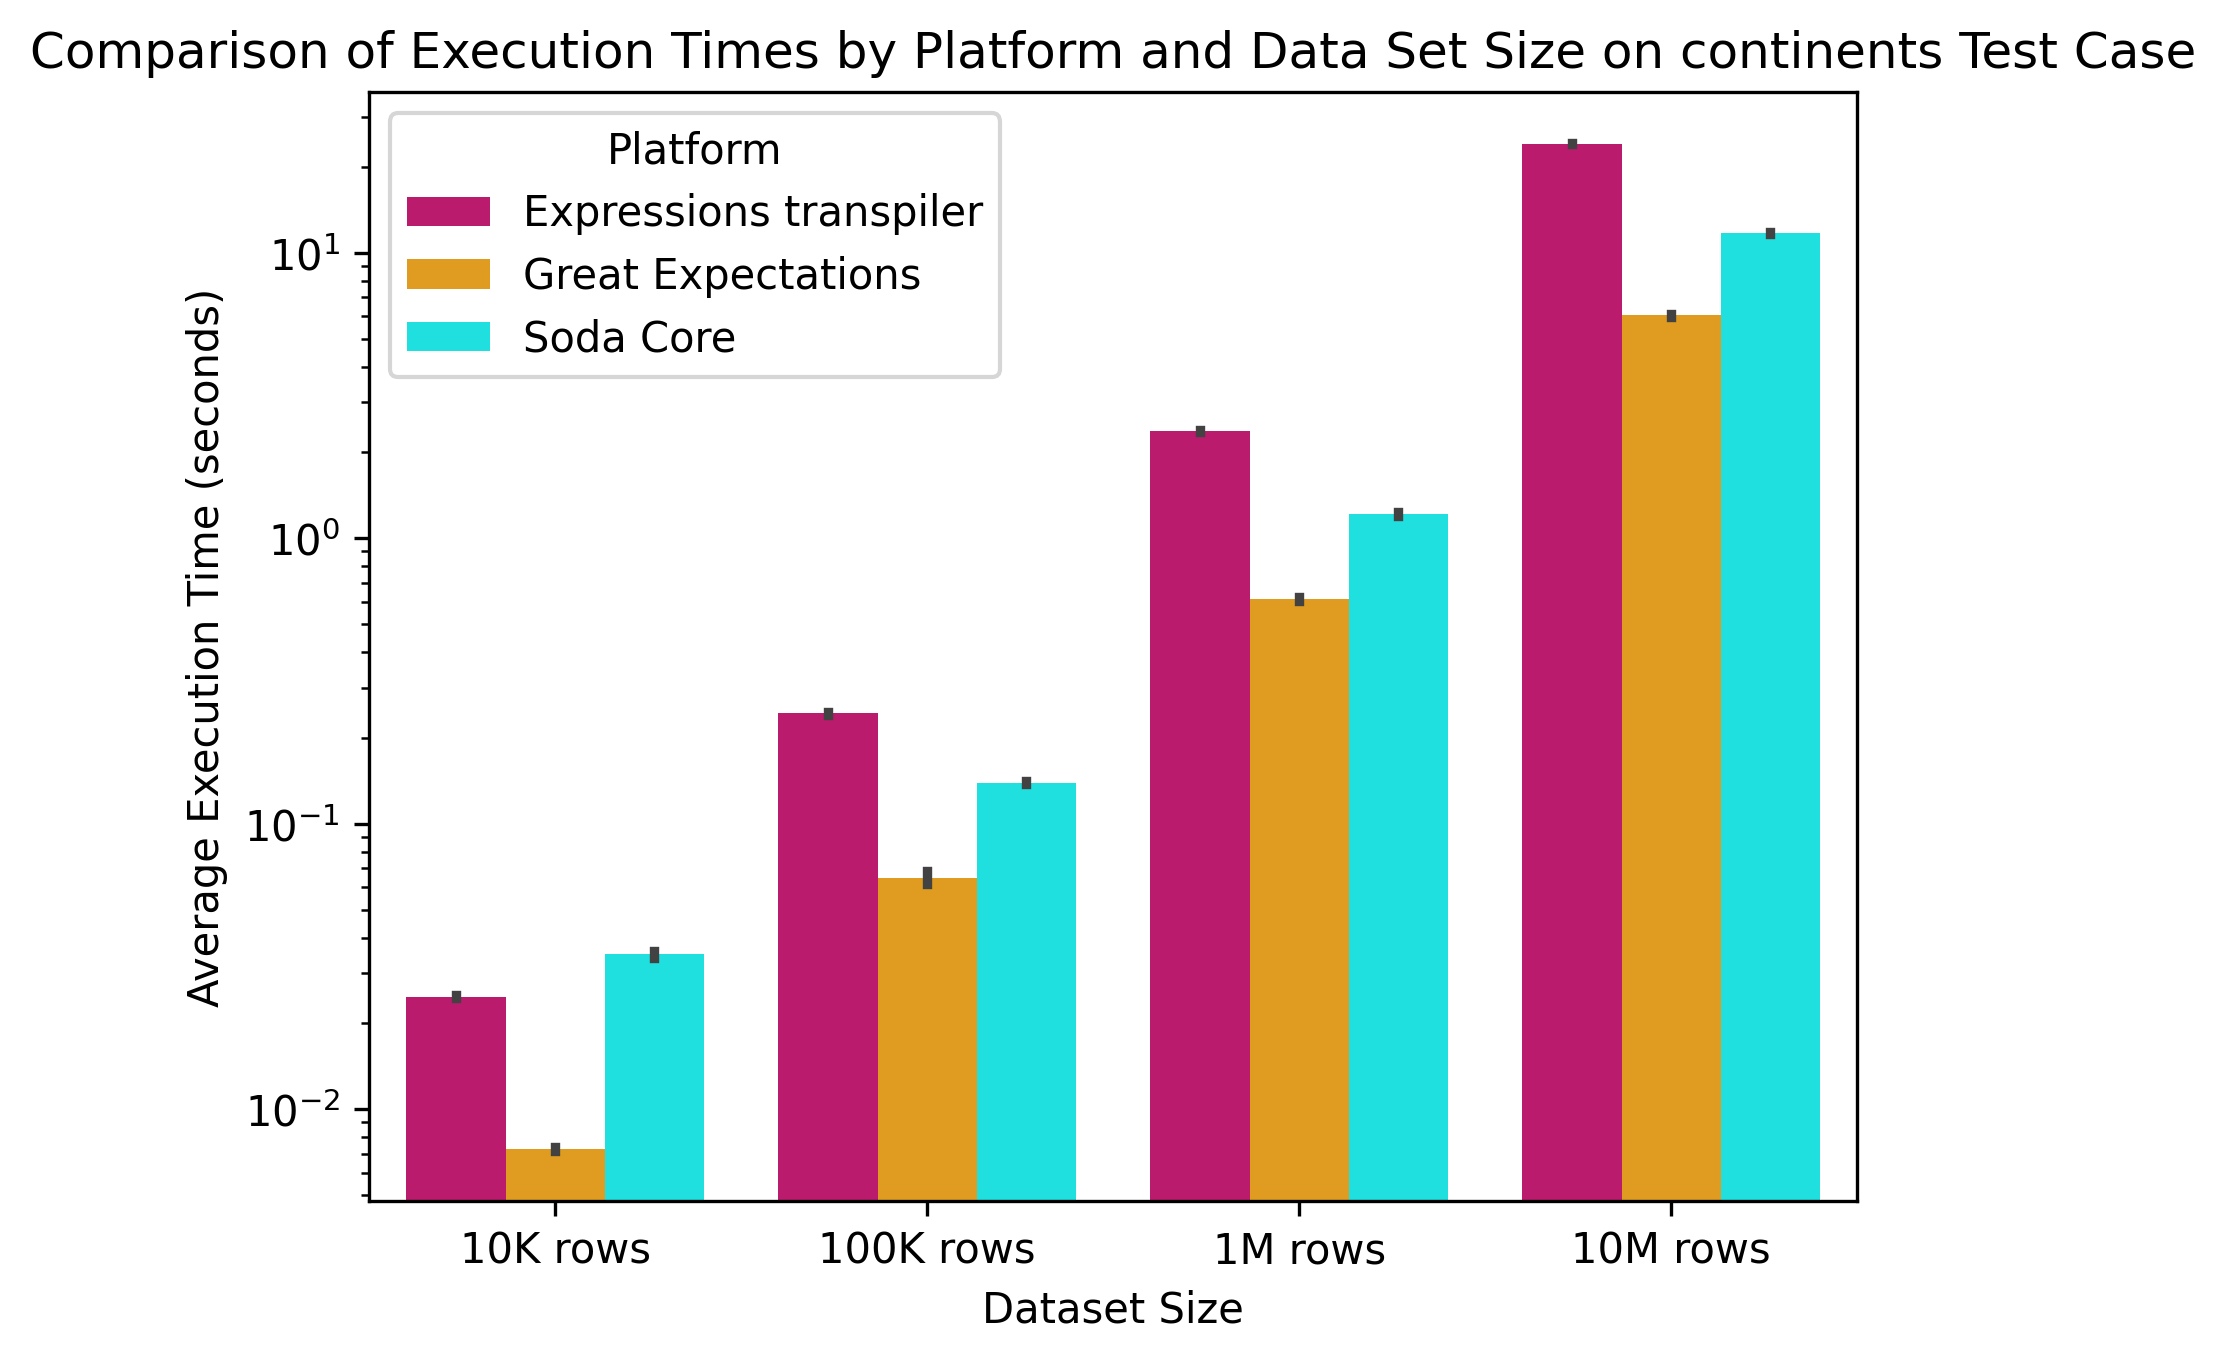
\includegraphics[width=1.0\columnwidth]{result-analysis/plots/execution_time_comparison_continents.png}
  \caption{Execution Time Comparison for test case n. 1: Continent Validation}
  \label{fig:time-comparison-continents}
\end{figure}


More important than the absolute execution time is the relative performance compared to the similar solutions. Table \ref{tab:time-continents} shows the relative execution time comparison to Soda Core for test case n. 1: Continent Validation. The results are also visualized in Figure \ref{fig:time-comparison-continents-relative}.

\begin{table}[h] 
  \centering 
  \caption{Relative execution time comparison to Soda Core for test case n. 1: Continent Validation} 
  \label{tab:time-continents-relative} 
  \begin{tabular}{llr}
\toprule
data set & platform & speedup relative to Soda Core \\
\midrule
10K rows & Great Expectations & 3.418893 \\
10K rows & Soda Core & -1.412433 \\
100K rows & Great Expectations & 3.762030 \\
100K rows & Soda Core & 1.747508 \\
1M rows & Great Expectations & 3.879196 \\
1M rows & Soda Core & 1.949125 \\
10M rows & Great Expectations & 3.998787 \\
10M rows & Soda Core & 2.055294 \\
\bottomrule
\end{tabular}

\end{table}

\begin{figure}[htbp]
  \centering
  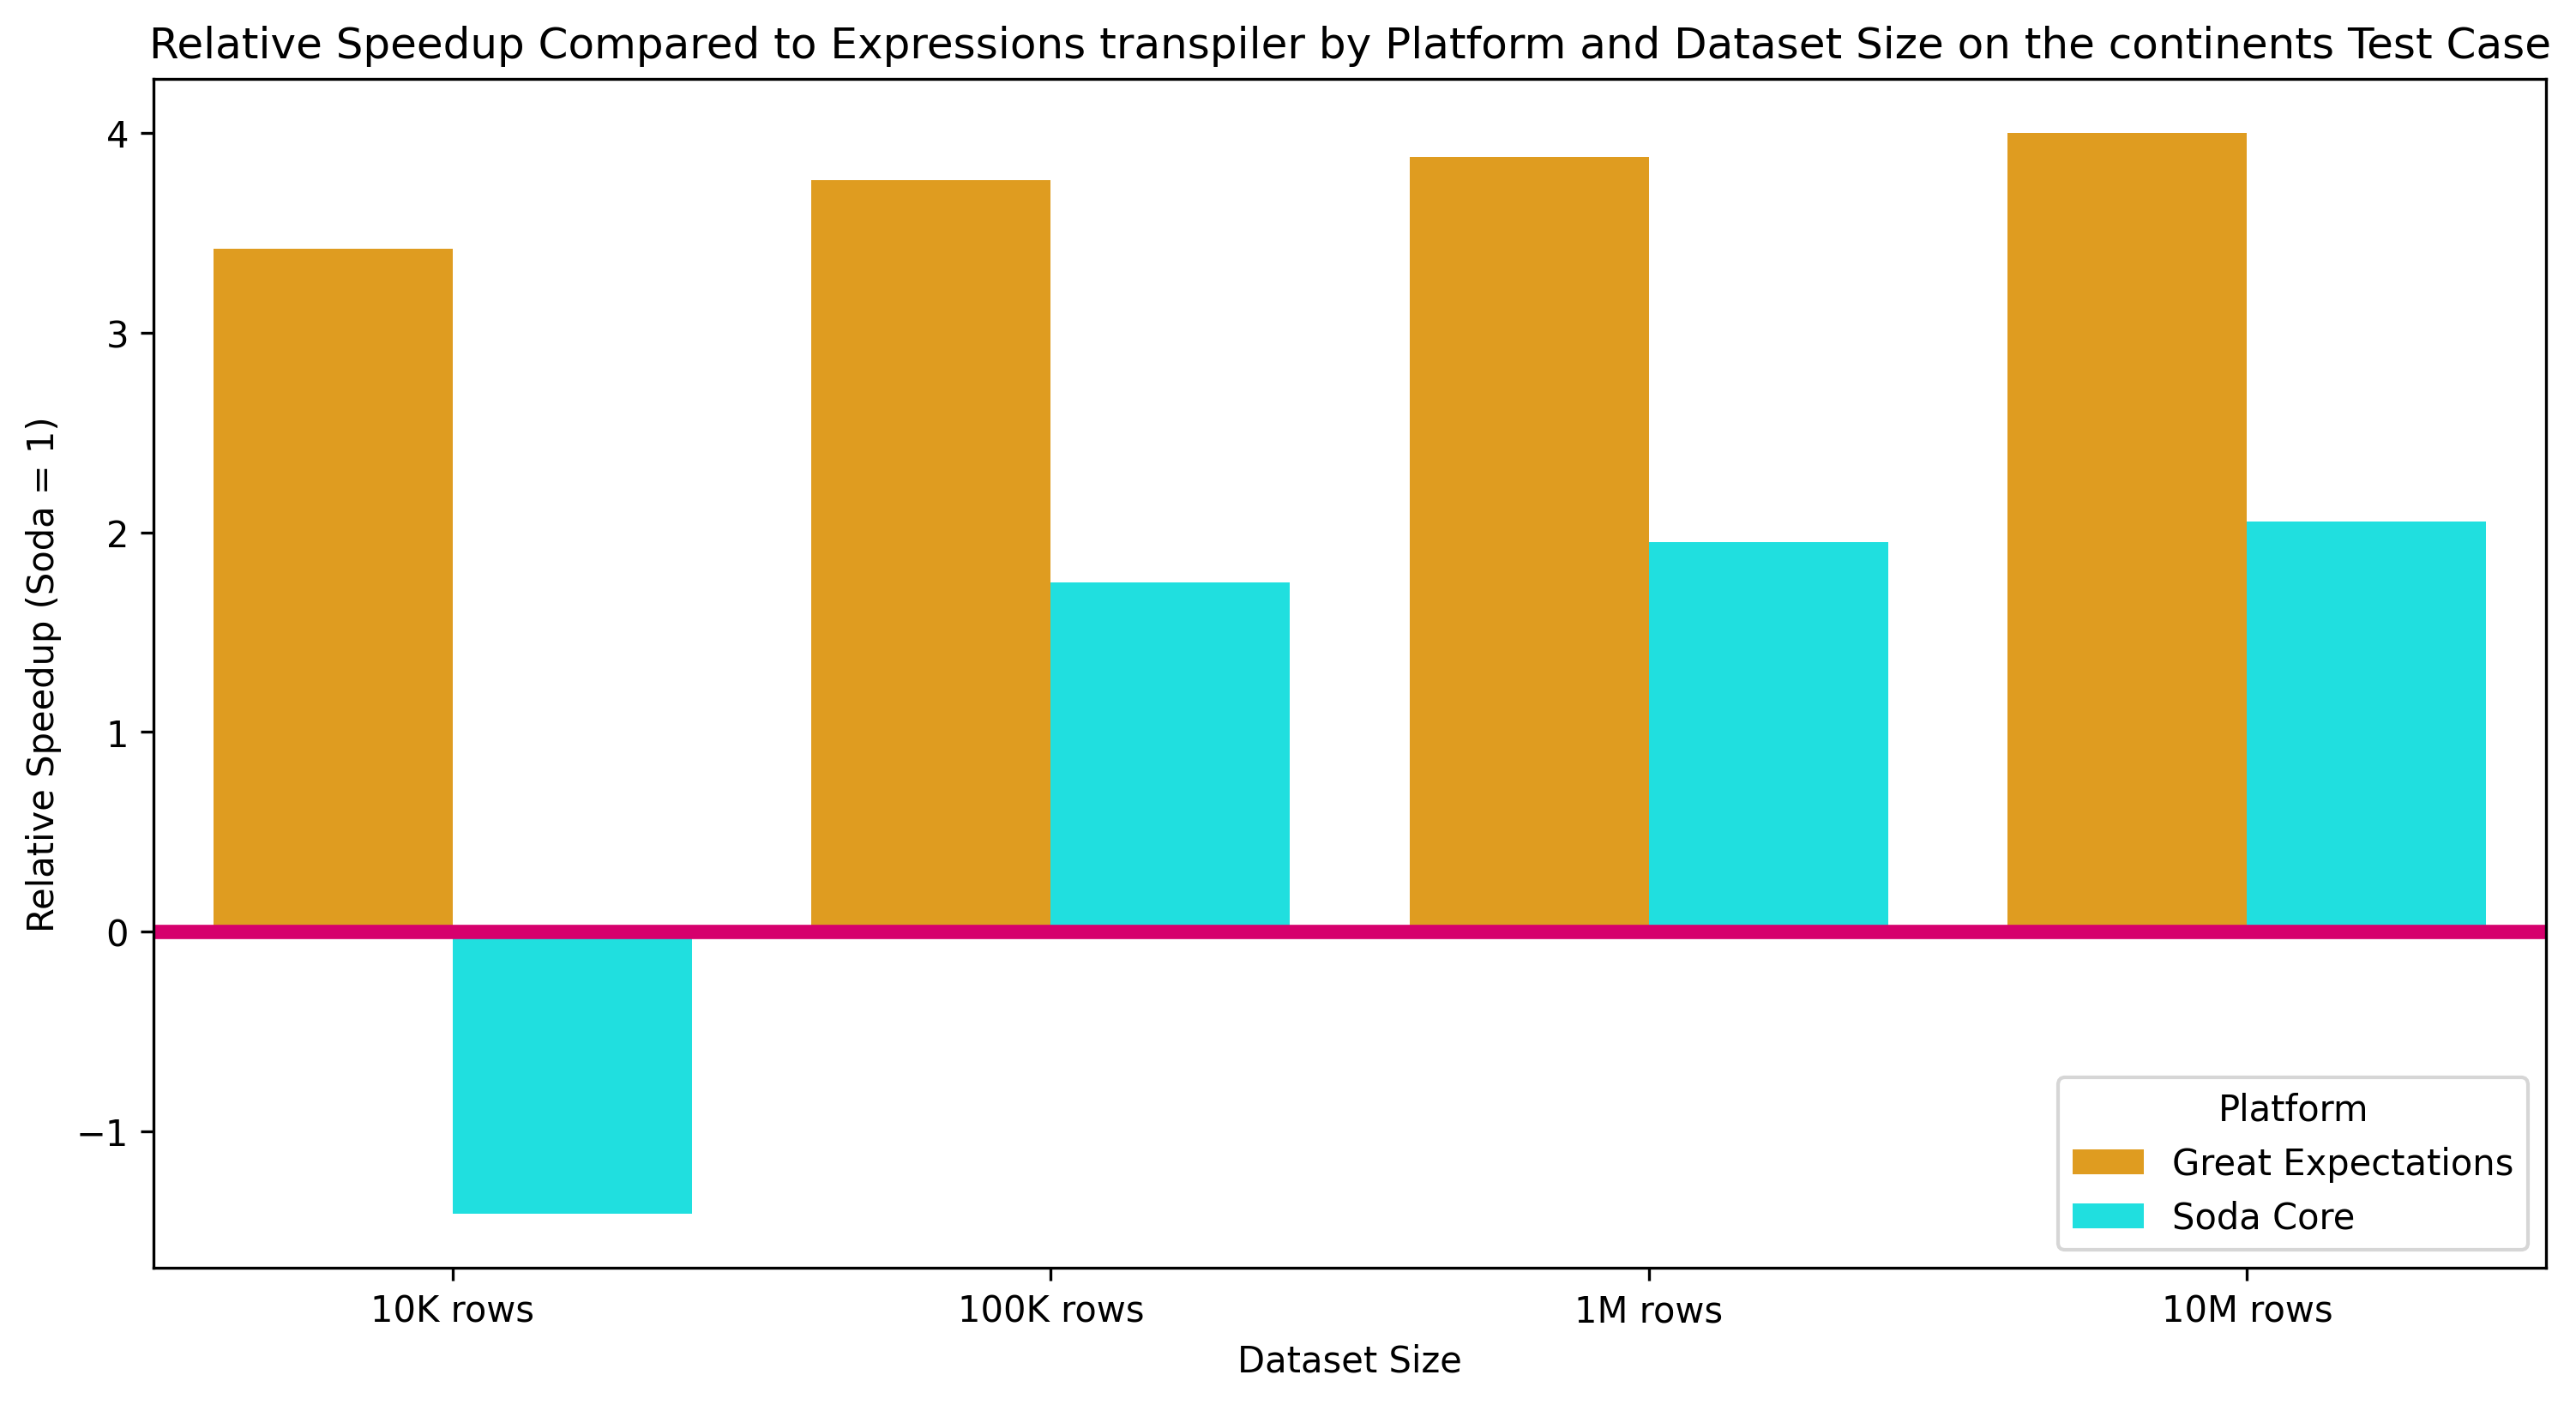
\includegraphics[width=1.0\columnwidth]{result-analysis/plots/relative_speedup_comparison_continents.png}
  \caption{Relative execution time comparison to Soda Core for test case n. 1. relative to Soda Core}
  \label{fig:time-comparison-continents-relative}
\end{figure}

In this simple test case, even for 10M records, the Python implementation is within an acceptable range of performance efficiency compared to the similar solutions. The execution time is slower than both Soda Core and Greater Expectations, but the difference is no more than 4x. 


\subsubsection{Test Case 2: Complex Customer Validation}

Table \ref{tab:time-customers} shows the execution time comparison for test case n. 2: Customers Validation. The results are also visualized in Figure \ref{fig:time-comparison-customers}.

\begin{table}[h] 
    \centering 
    \caption{Execution Time Comparison for test case n. 1: Continent Validation} 
    \label{tab:time-customers} 
    \begin{tabular}{llrr}
\toprule
data set & platform & mean execution time (s) & standard deviation (s) \\
\midrule
10K rows & Expressions transpiler & 0.766311 & 0.018873 \\
10K rows & Great Expectations & 5.909839 & 0.174845 \\
10K rows & Soda Core & 1.148130 & 0.033612 \\
100K rows & Expressions transpiler & 7.631781 & 0.125656 \\
100K rows & Great Expectations & 6.799458 & 0.140569 \\
100K rows & Soda Core & 2.405331 & 0.054677 \\
1M rows & Expressions transpiler & 76.628675 & 1.256378 \\
1M rows & Great Expectations & 12.591573 & 0.095586 \\
1M rows & Soda Core & 14.839434 & 0.100132 \\
\bottomrule
\end{tabular}

\end{table}

\begin{figure}[htbp]
  \centering
  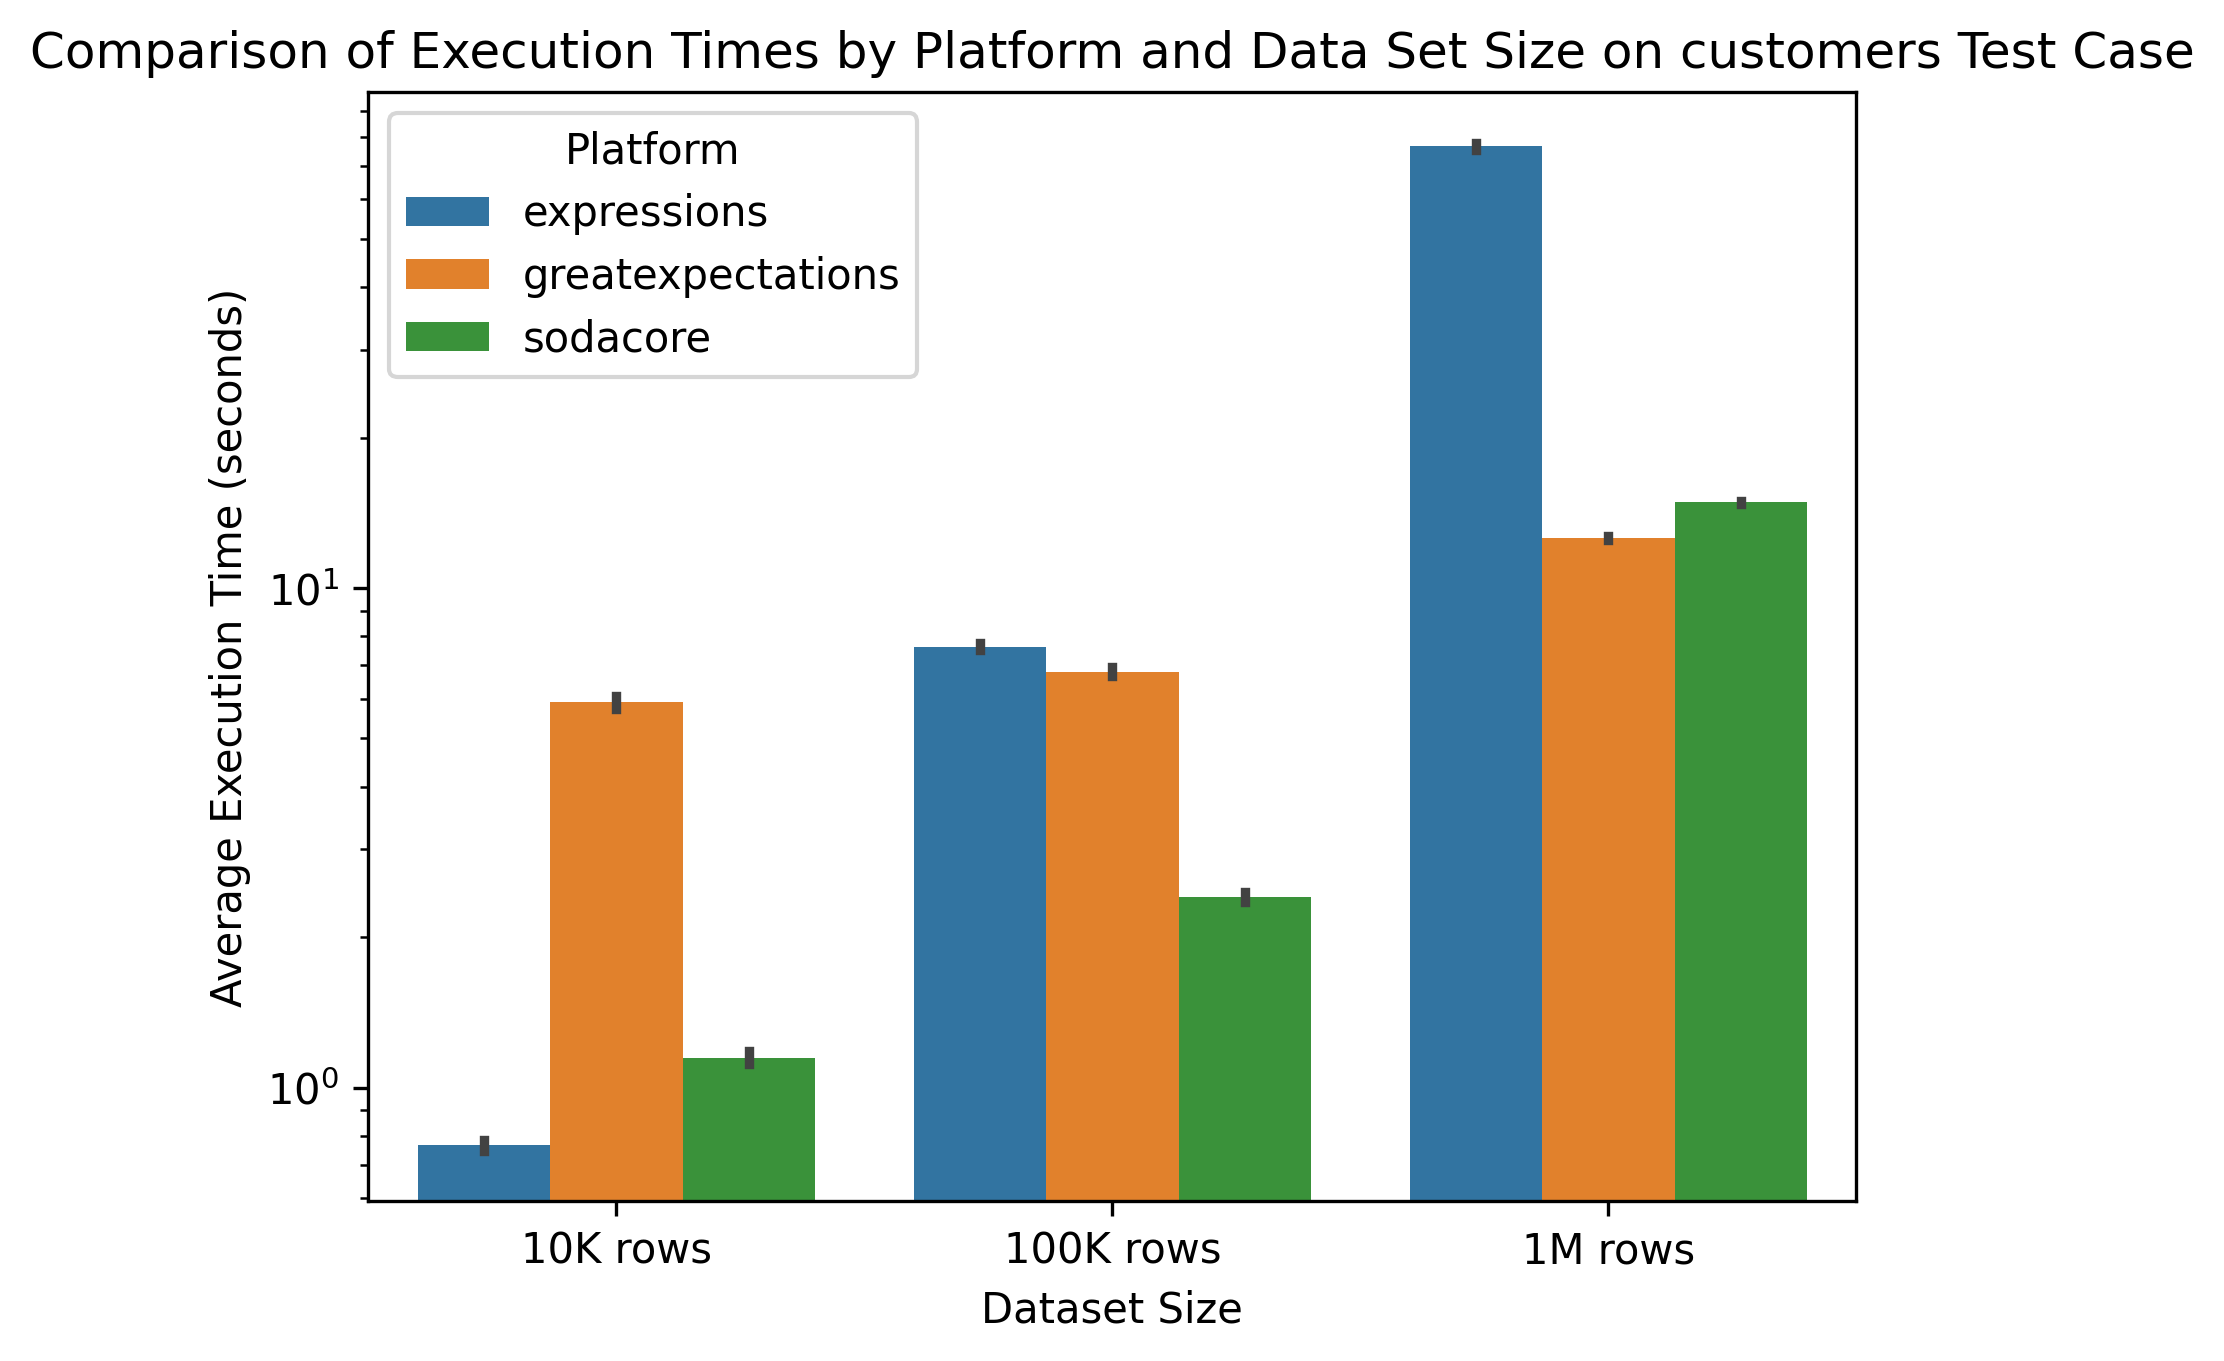
\includegraphics[width=1.0\columnwidth]{result-analysis/plots/execution_time_comparison_customers.png}
  \caption{Execution Time Comparison for test case n. 2: Customer Validation}
  \label{fig:time-comparison-customers}
\end{figure}


More important than the absolute execution time is the relative performance compared to similar solutions. Table \ref{tab:time-customers} shows the relative execution time comparison to Soda Core for test case n. 1: Continent Validation. The results are also visualized in Figure \ref{fig:time-comparison-customers-relative}.

\begin{table}[h] 
  \centering 
  \caption{Relative execution time comparison to Soda Core for test case n. 2: Customer Validation} 
  \label{tab:time-customers-relative} 
  \begin{tabular}{llr}
\toprule
data set & platform & speedup relative to the Python transpiler \\
\midrule
10K rows & Great Expectations & 0.129667 \\
10K rows & Soda Core & 0.667443 \\
100K rows & Great Expectations & 1.122410 \\
100K rows & Soda Core & 3.172861 \\
1M rows & Great Expectations & 6.085711 \\
1M rows & Soda Core & 5.163854 \\
\bottomrule
\end{tabular}

\end{table}

\begin{figure}[htbp]
  \centering
  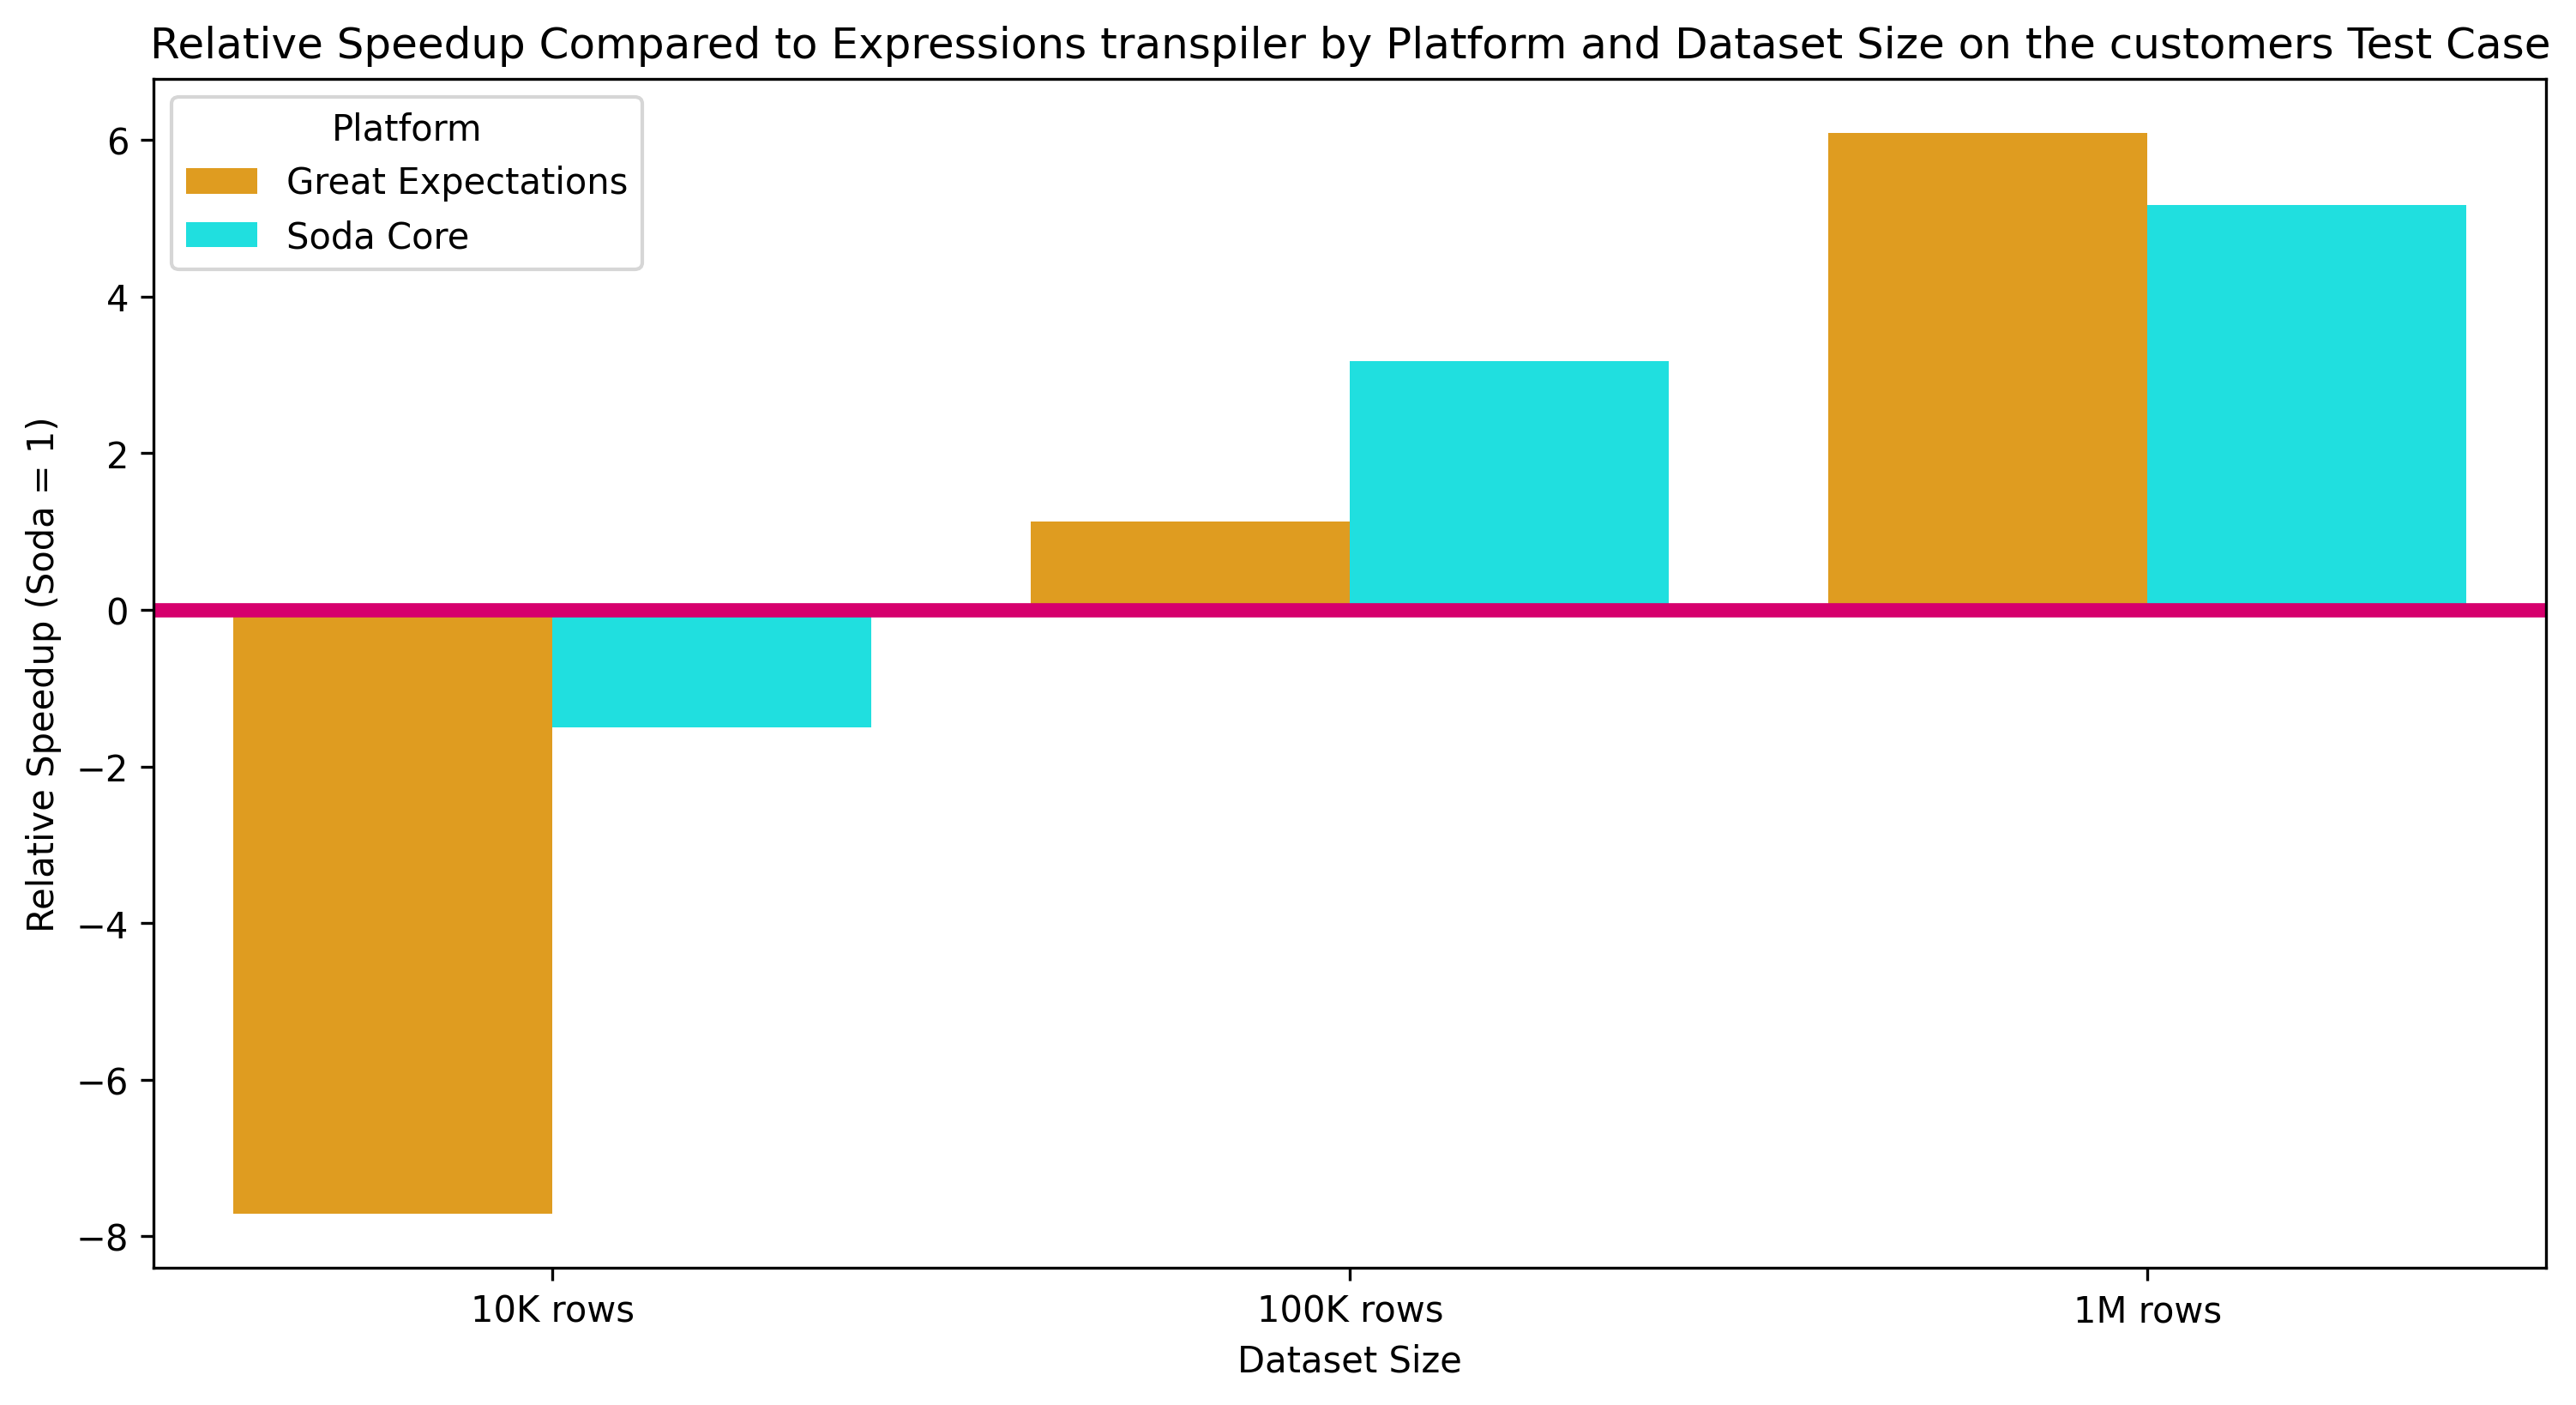
\includegraphics[width=1.0\columnwidth]{result-analysis/plots/relative_speedup_comparison_customers.png}
  \caption{Relative execution time comparison to Soda Core for test case n. 2. relative to Soda Core}
  \label{fig:time-comparison-customers-relative}
\end{figure}

In the more complex test case involving reference data lookups, even for 1M records, the Python implementation is within an acceptable range of performance efficiency compared to the similar solutions. The execution time is slower than for both Soda Core and Greater Expectations, but the difference is below 10x. 

\section{Discussion}

%     Interpretation of Results: Discuss the implications of the test results for the viability of the Python implementation in real-world applications.
%     Potential Bottlenecks and Limitations: Identify any performance bottlenecks or limitations observed during testing and suggest possible explanations or solutions.

The performance analysis of the Python implementation of the Ataccama Expression Language reveals that the system is within an acceptable range of performance efficiency for real-world applications. The Python version, while slower than similar tested solutions Soda Core and Great Expectations, remains competitive in terms of execution time, even for large datasets. The performance results indicate that the Python implementation can handle data quality rules efficiently and effectively, making it a viable alternative for data engineers who require programmatic access to Ataccama's data quality tools.

The performance gap is acceptable, especially considering the more comprehensive feature set it provides compared to the other two solutions. 




